%!TEX root = ../main.tex
\part{Data Analyses}
\label{chap:TimingAHCAL}

\chapter{AHCAL Testbeam setup \& Event Selection}
\label{chap:EvtSelection}

%%% Need to rethink about this...
The experimental data used in this thesis has been collected in a testbeam campaign at the SPS facility at CERN in July 2015 with the AHCAL technological prototype described in section \ref{sec:AHCAL}.

The main topic of this thesis is the study of the \textit{time development of hadronic showers} and the study of the \textit{effects of timing cuts} in a hadronic calorimeter. The analysis is divided in several part. In the first part, the energy scale calibration of the AHCAL prototype is presented in chapter \ref{chap:ECalibAHCAL}. In the second part, the timing calibration of the AHCAL is presented in chapter \ref{chap:TimingCalib}. In a third part, the cross-check of the time calibration and the validation of the simulation is shown in chapter \ref{chap:TimingValidation}. Finally, the analysis of the recorded pion data is described in chapter \ref{chap:TimingPions}.

This chapter discusses the setup of the testbeam first before presenting the selected dataset for this analysis, the selection of the triggers needed for this analysis as time reference and the selection criteria for each dataset of muons, electrons and pions.

\section{Testbeam Configuration}

\subsection{Beamline Setup}
\label{sec:beamline}

During the summer of 2015, the CALICE collaboration performed several testbeam campaigns with the AHCAL technological prototype. The detector was installed in the beamline H2 in the SPS North Area at CERN \cite{H2Beamline}. This beamline is equipped with wire chambers and scintillators that provide information of the beam position and number of particles. The wire chamber information would have been useful in order to simulate correctly the beam profile. Unfortunately, this information could not be recorded with the AHCAL data acquisition system. The information available about the amount of material upstream of the detector until the last momentum selection magnet is limited thus the simulation of the beamline is simplified.

A Cherenkov detector (at around 100 m upstream) was available to tag incoming particles. These detectors take advantage of the fact that, a particle that traverses a medium faster than the speed of light in that medium will generate a cone of Cherenkov light. The opening angle of the cone is proportional to the particle mass \cite{GOVORKOV20059}. The Cherenkov detector at this beamline offered the possibility to set a threshold for particle tagging. This is particularly needed to tag possible contaminating electrons in a pion beam. The tagging signal from the Cherenkov detector was provided directly to several AHCAL channels.

For the production of particles, a primary high-intensity proton beam (around $10^{12}$ protons per burst) of 400 GeV impinges on a target. From this, a secondary beam is produced containing various particle types and energies.

A muon beam can be obtained from the decay of a collimated pion beam which are stopped by a collimator before the last bending magnet.

For electrons, a neutral beam of photons is directed to a lead target to generate electrons from gamma conversion, producing a very pure electron beam. Another possibility is to impinge a charged beam onto a secondary target and filter the beam with an absorber. But this has the disadvantage of low rates at low energy and possible contamination of the electron beam with pions \cite{H2Beamline}.

For pions, the momentum is selected via a set of collimators and magnets. Due to the decay of $\pi_0$ (conversion of the photons into the absorber filter) and the acceptance of the beamline, a contamination of the pion beam with electrons is possible at low momentum (< 20 GeV).

\subsection{Testbeam Setup}
\label{sec:TBsetup}

In July 2015, the AHCAL detector was using the full EUDET steel stack \cite{EUDET-Report-2010-02} with 48 iron absorber plates. In the stack, 14 active layers are installed. The detector is placed on a movable stage in order to be able to move the detector position relative to the beam for muon calibration runs. A simplified view of the beamline configuration is shown in figure \ref{fig:TestbeamScketch}.

\begin{figure}[htbp!]
	\centering
	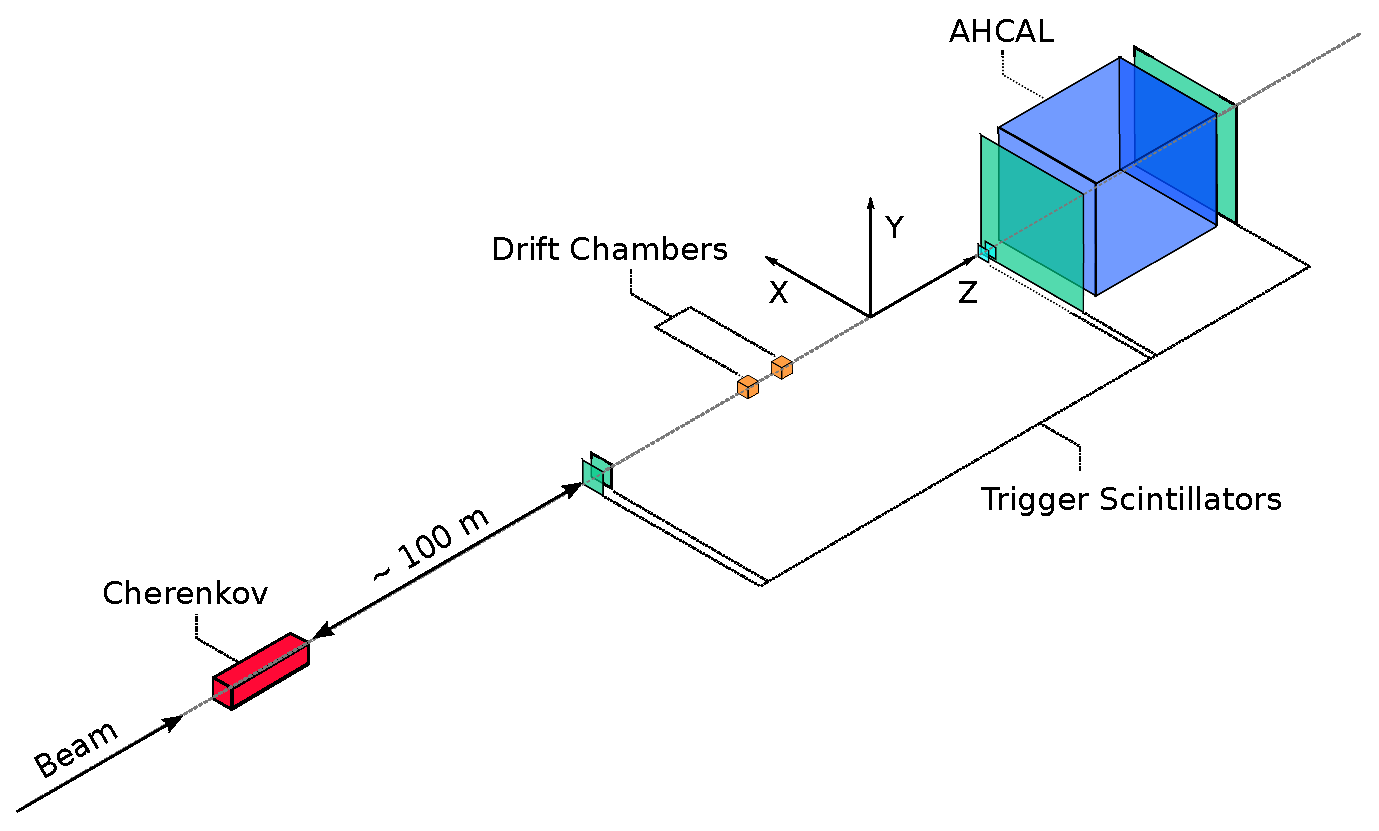
\includegraphics[width=0.7\linewidth]{chap5/fig_EnergyCalib/TestbeamSetup.eps}
	\caption{Sketch view of the beamline setup at the CERN SPS H2 beamline in July 2015.} \label{fig:TestbeamScketch}
\end{figure}

\begin{figure}[htbp!]
	\centering
	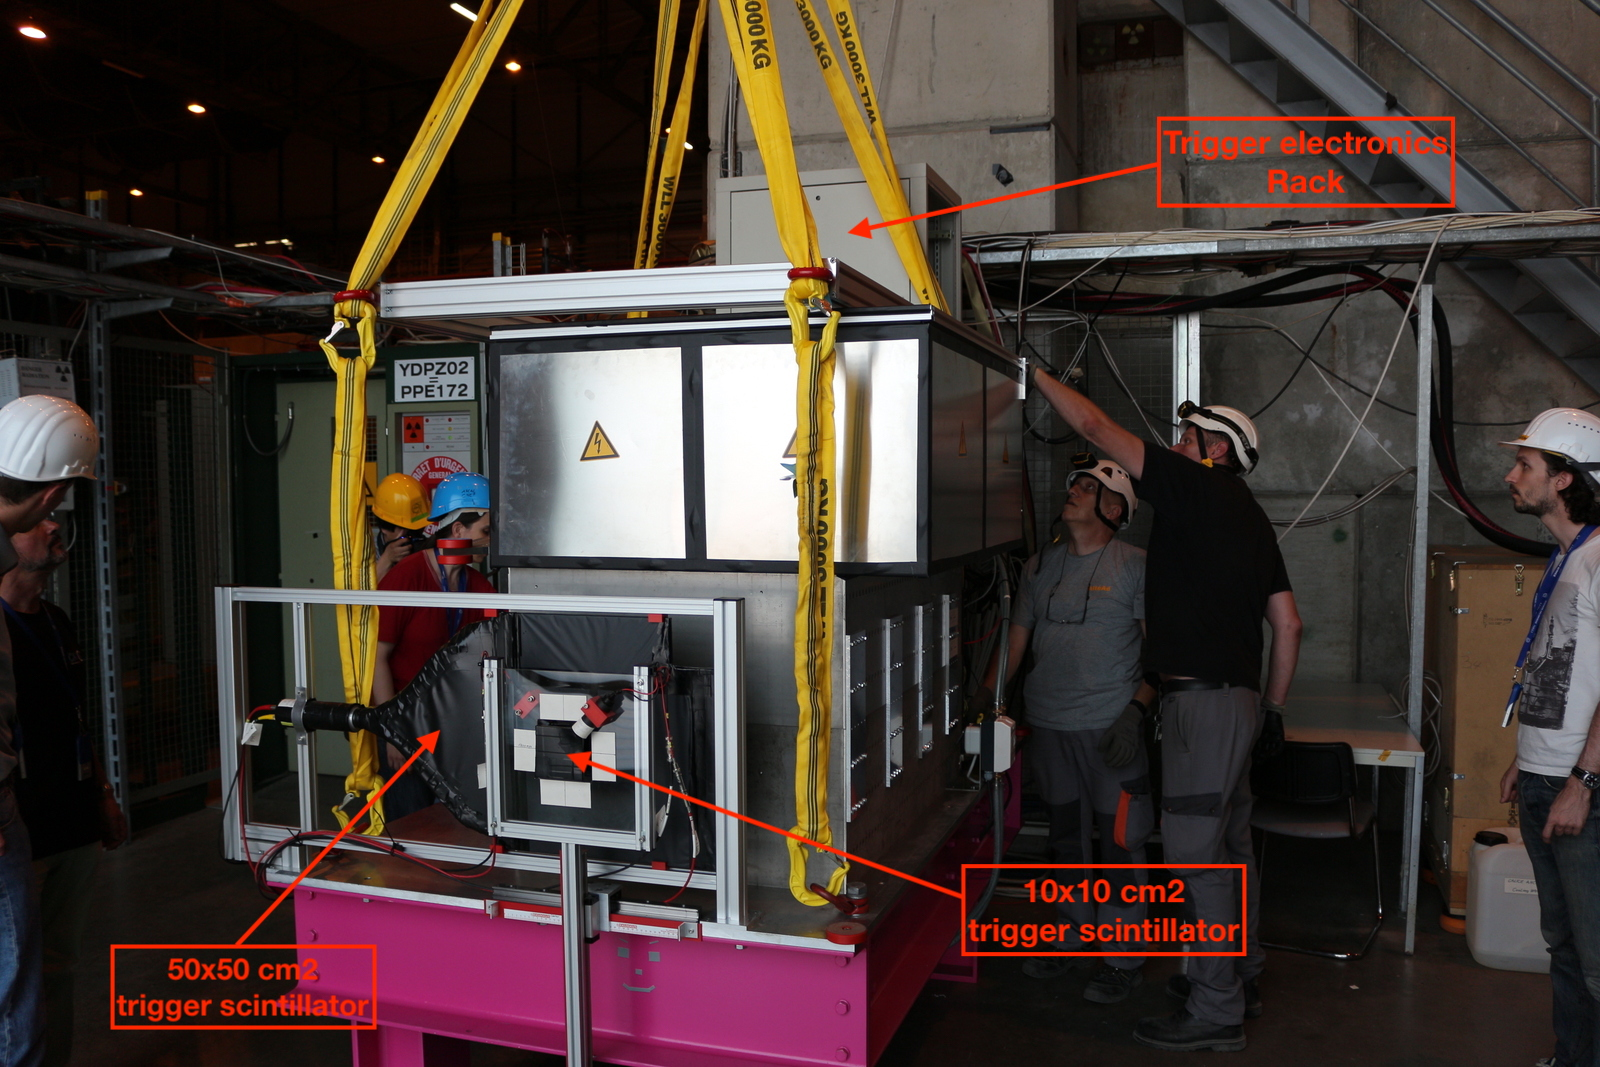
\includegraphics[width=0.7\linewidth]{chap5/fig_EnergyCalib/IMG_1170_copy.jpg}
	\caption{Photo of the AHCAL detector during the installation in the testbeam area.} \label{fig:AHCAL_photo}
\end{figure}

The beam instrumentation consists of two $10\times10$ cm$^2$ scintillator plates in front of the calorimeter, and two $50\times50$ cm$^2$ scintillator plates, one placed in front of the calorimeter and one placed at the back of the calorimeter as shown in figure \ref{fig:AHCAL_photo}. They are read-out by photomultiplier tubes. The coincidence of the $50\times50$ cm$^2$ scintillator plates is used for the muon runs and the coincidence of the $10\times10$ cm$^2$ scintillator plates is used for the electron and pion runs as a trigger signal.

Additionally, the coincidence signal from the scintillator is provided directly to several channels of the AHCAL in order to provide a reference time information of the trigger which is important for the timing study presented in this thesis. A simplified view of the layer structure of the AHCAL is shown in figure \ref{fig:Det_layout}.

\begin{figure}[htbp!]
	\centering
	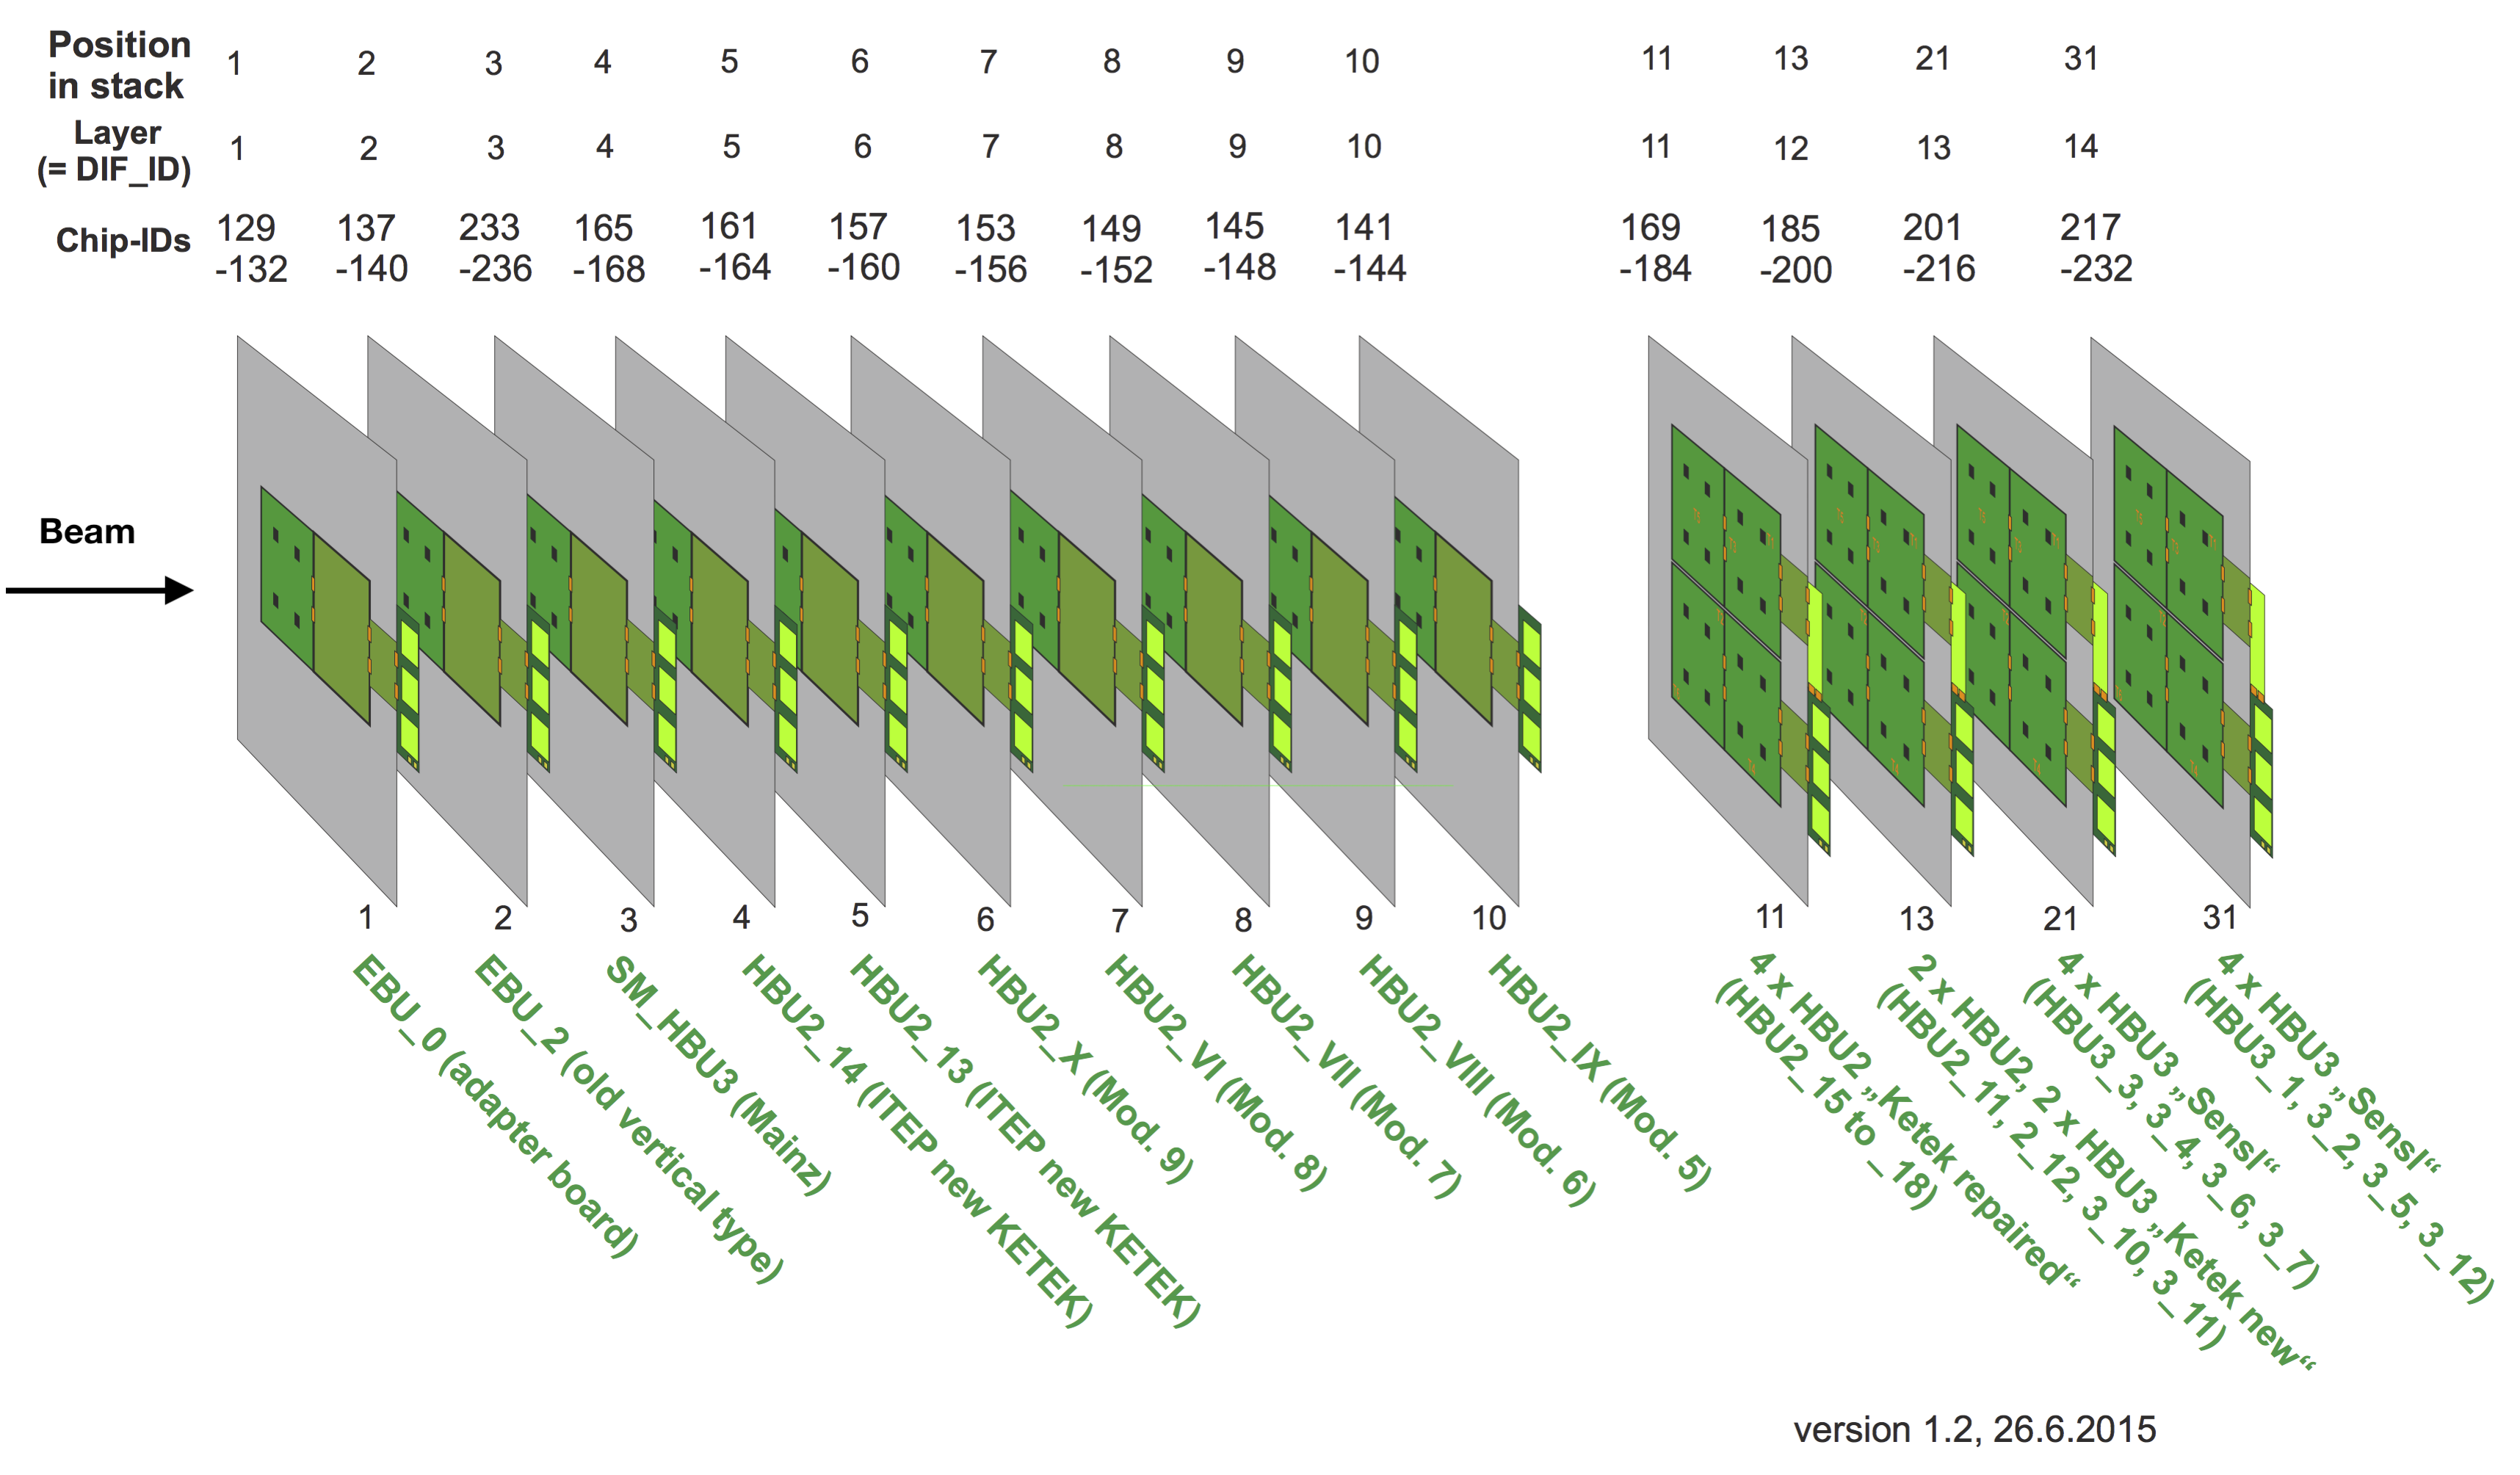
\includegraphics[width=0.7\linewidth]{chap5/fig_EnergyCalib/Detector_layout_copy.png}
	\caption{Simplified view of the detector layout used in July 2015.} \label{fig:Det_layout}
\end{figure}

\subsection{Time reference}
\label{subsec:trigger}

The scintillator plates are used as a time reference signal. Both type of scintillator are connected to a discriminator and a gate for coincidence in order to provide a validation signal to the readout chip (see section \ref{sec:SPIROC2B}).

When a coincidence happens, a signal of 4 $\mu$s length with a fast rising edge of around 1 ns, is generated with an amplitude around 100 mV that is used as a time reference. This signal is provided \textit{directly to six AHCAL channels} for redundancy. The list of the AHCAL channels used as a reference time are shown in table \ref{table:trigger_signal_list}. No other external time reference is available.

\begin{table}[htb!]
	\centering
	\caption{List of AHCAL channels used as time reference for this analysis.}
	\label{table:trigger_signal_list}
	\begin{tabular}{@{} ccccc @{}}
		\toprule
		Layer \# & Chip Number & Channel & Comments & Name \\
		\midrule
		11 & 169 & 29 & noisy & T$_{11}$ \\
		11 & 177 & 23 & broken & - \\
		12 & 185 & 29 & - & T$_{12}$ \\
		13 & 201 & 29 & -  & T$_{13}$ \\
		13 & 211 & 6 & broken & - \\
		14 & 217 & 23 & - & T$_{14}$ \\
		\bottomrule
	\end{tabular}
\end{table}

In the following analysis, the time reference signals T$_{12}$, T$_{13}$ and T$_{14}$ are used. The channels are determined to be noisy or broken by looking at the energy spectra of these channels. Broken channels results in an empty energy spectrum and noisy channels are showing two energy peaks, one near the pedestal and another at the expected energy value. The channel T$_{11}$ is not used as it presented a very low efficiency due to noise.

\section{Dataset and Event Selection}

The selections presented in this section are based on simulated data. Beforehand, the simulation has been carefully validated and represents within 10-20\% the data in muon and electron beam. More details can be seen in section \ref{sec:SimulationVal}.

\subsection{Dataset}
\label{subsec:dataset}

During the campaign at the CERN \acrshort{sps} facility in July 2015, firstly, muon runs were taken at beam energies of 50 GeV and 150 GeV for calibrating the detector. Secondly, several electron runs were taken at beam energies between 10 GeV and 50 GeV to study the electromagnetic response of the calorimeter. Finally, the pion runs were taken at beam energies between 10 GeV and 90 GeV.

The table \ref{table:dataruns} sums up the datasets taken in different beams. The number of events shown in the table is the total number of recorded events.

\begin{table}[htb!]
	\centering
	\caption{List of runs taken at SPS in July 2015.}
	\label{table:dataruns}
	\begin{tabular}{@{}lp{2cm}p{7.5cm}p{2cm}@{}}
		\toprule
		\multicolumn{1}{l}{\textbf{Particle}} & \textbf{Energy} & \textbf{Runs} & \textbf{\# Events}\\
		\midrule
		\multirow{2}{*}{$\mu^-$}& 50 GeV & 24016-24204 & 120,887,651\\& 150 GeV & 24623-24662 & 15,534,328\\
		\midrule
		\multirow{2}{*}{e$^-$}& 10 GeV & 24531-24576 & 38,028,438\\& 15 GeV & 24507-24527 & 7,701,325\\& 20 GeV & 24479-24504 & 10,498,554\\& 30 GeV & 24454-24475 & 3,382,943\\& 40 GeV & 24420-24448 & 2,665,843\\& 50 GeV & 24404-24419 & 5,933,995\\
		\midrule
		\multirow{2}{*}{$\pi^-$}& 10 GeV & 24266-24272, 24300-24317, 24381-24397 & 24,311,420\\& 20 GeV & 24398-24400 & N/A\\& 30 GeV & 24259-24299, 24319-24380 & 10,120,753\\& 50 GeV & 24212-24254, 24325-24357, 24580-24612 & 10,704,661\\& 70 GeV & 24219-24242, 24365-24374 & 8,885,407\\& 90 GeV & 24233-24287, 24331-24364 & 7,955,604\\
		\bottomrule
	\end{tabular}
\end{table}

\subsection{Muon selection}
\label{subsec:Muon_presel}

\subsubsection{Pre-selection}

A clean selection of MIP-like particles is needed in order to obtain and cross-check the energy scale calibration of the AHCAL (see chapter \ref{chap:ECalibAHCAL}) and as well performing the timing calibration of the detector (see chapter \ref{chap:TimingCalib}) at a single cell level. A simple pre-selection was performed on the muon dataset designed to select MIP-like particles going through the AHCAL. In a second step, a track selection was performed to retain only MIP-like particle as explained in section \ref{subsec:Muon_sel}.

The pre-selection is based on the energy weighted center of gravity along the beam axis $cog_Z = \frac{\Sigma{i} E_i z_i}{\Sigma_{i} E_i}$ and the number of hits $n_{Hits}$. A MIP-like particle should, in principle, deposit the same energy in each layer of the calorimeter thus $cog_Z$ should be roughly centered in the calorimeter in the z coordinate. In addition, the number of hits should be around 1 per layer for a MIP-like particle plus the number of noise hits expected in the detector, therefore explaining a cut at $n_{Hits} = 20$.

The distribution in the plane $cog_Z$:$n_{Hits}$ shown in figure \ref{fig:Muons_CoGZ_nHits} is obtained from simulated 150 GeV muons, electrons and pions. The applied pre-selection is represented by the black box. The pre-selection removes few muon events, as well as it discards electrons greatly and rejects also a large fraction of pions. The pre-selection efficiency is 99.4\% for muons, 0\% for electrons and 13.3\% for pions.

\begin{figure}[htbp!]
	\centering
	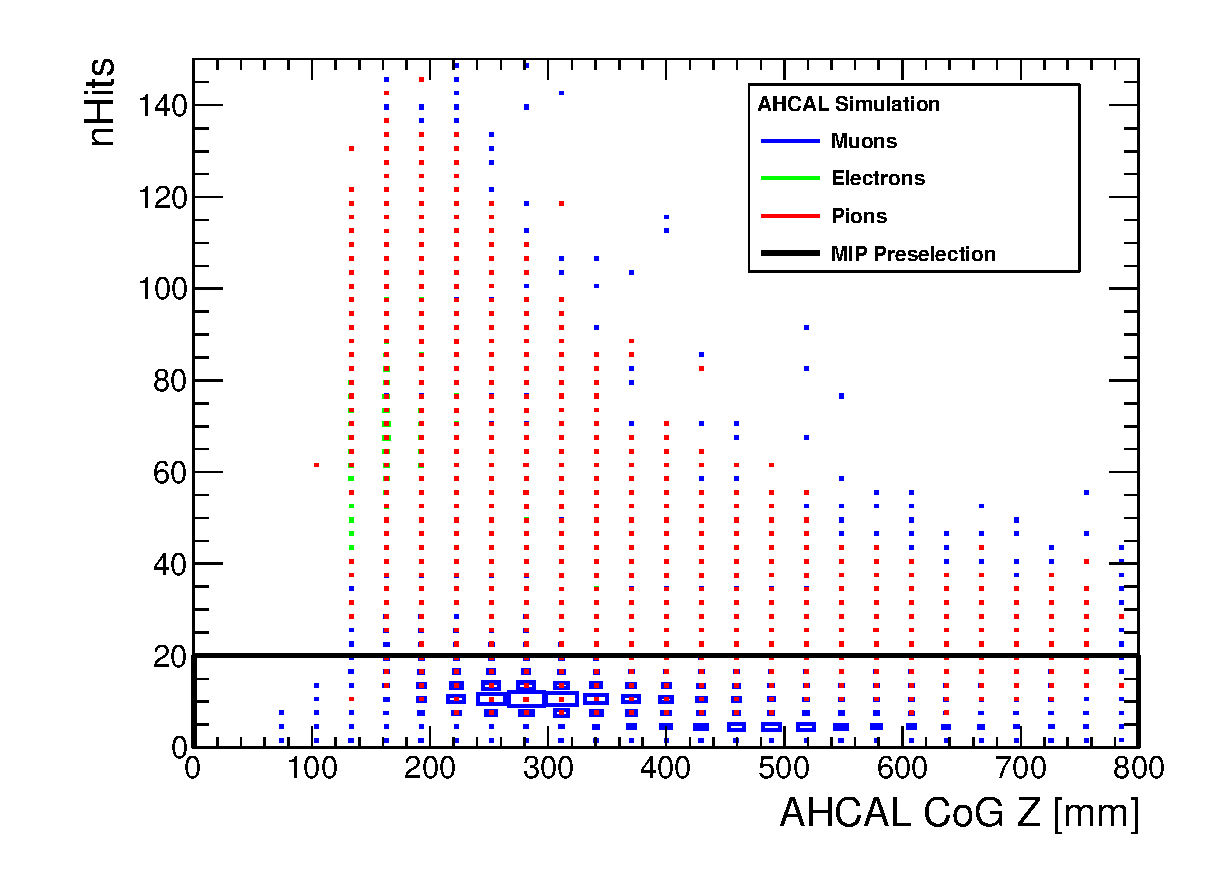
\includegraphics[width=0.7\linewidth]{../Thesis_Plots/Timing/Muons/Plots/SelectionCut_nHitsCoGZ_Muons.eps}
	\caption{Event distribution in $cog_Z:n_{Hits}$ plane. The size of each box represents the number of events in each bin. The black box represents the space-phase covered by the pre-selection.} \label{fig:Muons_CoGZ_nHits}
\end{figure}

\subsubsection{Selection}
\label{subsec:Muon_sel}

By looking at the spectrum of the number of hits per event, it is estimated that around 30\% of the events in the muon runs are contaminated by pions.

The MIP selection was designed to efficiently select muons and reject late pion showers. For this, a MIP track finder has been developed based on previous work \cite{Hartbrich:2016bbz}. This algorithm is designed to select MIP-like particle tracks in the AHCAL detector and remove pion showers.

The algorithm selects AHCAL towers of hits in the same $x:y$ position and it rejects AHCAL towers that contains less than a certain number of hits. In order to select muons or punch-through pions, a straight track of at least 7 hits is required in the whole AHCAL. This assumes that the calorimeter was perfectly perpendicular to the beam, therefore any tilted tracks would be missed. In addition, to reject late pion showers, no more than 2 hits are allowed per layer to account for some flexibility with noise hits.

The distributions of the maximum number of hits in a layer and the number of hits of a track are shown in figures \ref{fig:Muons_Track_nHitsLayer} and \ref{fig:Muons_Track_nHits} for simulated samples of 150 GeV muons, electrons and pions after pre-selection. The MIP track finder was performed in two steps for the inner part of the detector of $12 \times 12$ tiles and the outer part for the big layers (layers 11 to 14, Outer BL) in order to calibrate the outer channels of these layers. The figure \ref{fig:Muons_Track_nHitsLayer} shows that a cut of two hits per layer is optimal in order to reject pions without affecting muons too much.

The selection efficiency is 72.5\% for muons, 0\% for electrons and 5.6\% for pions. The selection reduces further the pion contamination and the remaining pion fraction is compatible with the fraction of pions traversing the AHCAL without hard interaction. An overview of the MIP selection cuts is given in table \ref{table:muon_sel}.

\begin{figure}[htbp!]
	\begin{subfigure}[t]{0.49\textwidth}
		\centering
		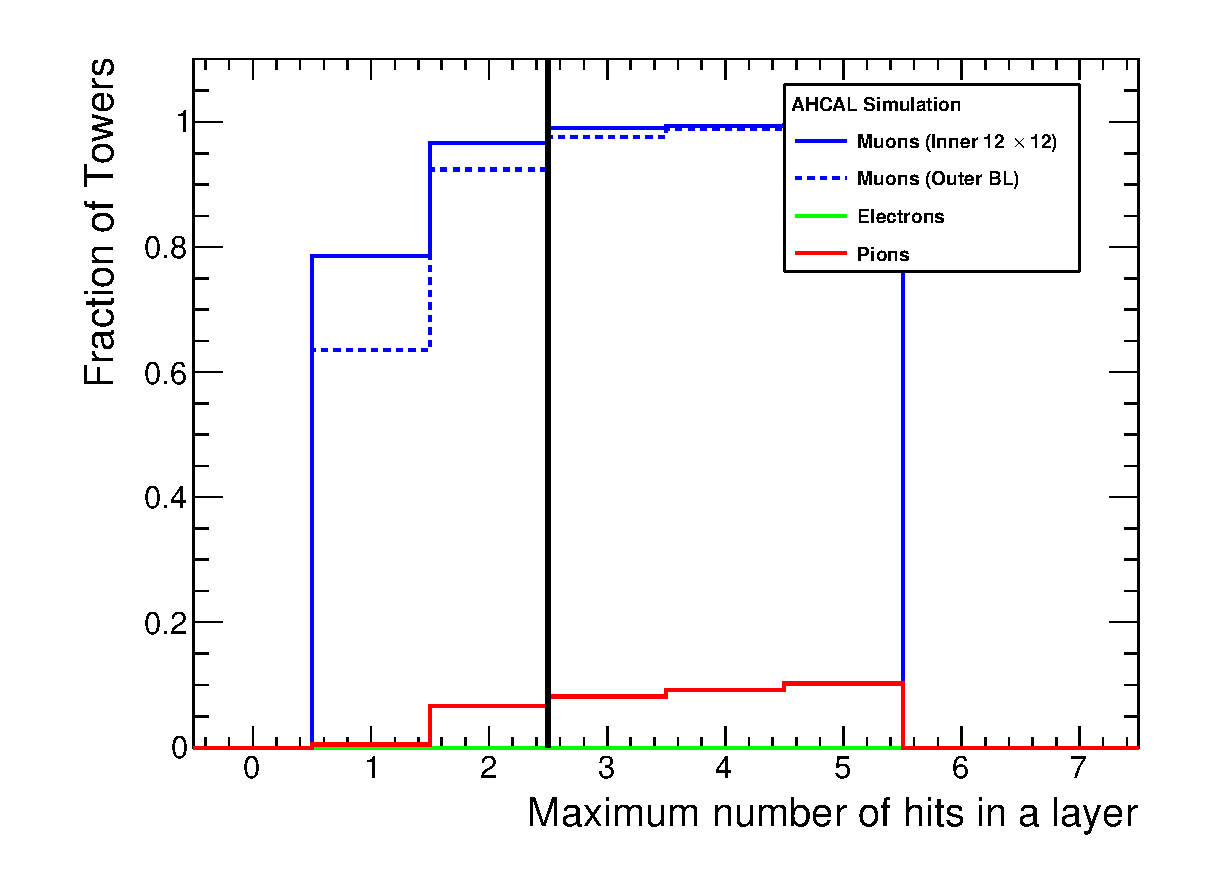
\includegraphics[width=1\linewidth]{../Thesis_Plots/Timing/Muons/Plots/TrackFinderCut_nHitsLayer_Muons.eps}
		\caption{} \label{fig:Muons_Track_nHitsLayer}
	\end{subfigure}
	\hfill
	\begin{subfigure}[t]{0.49\textwidth}
		\centering
		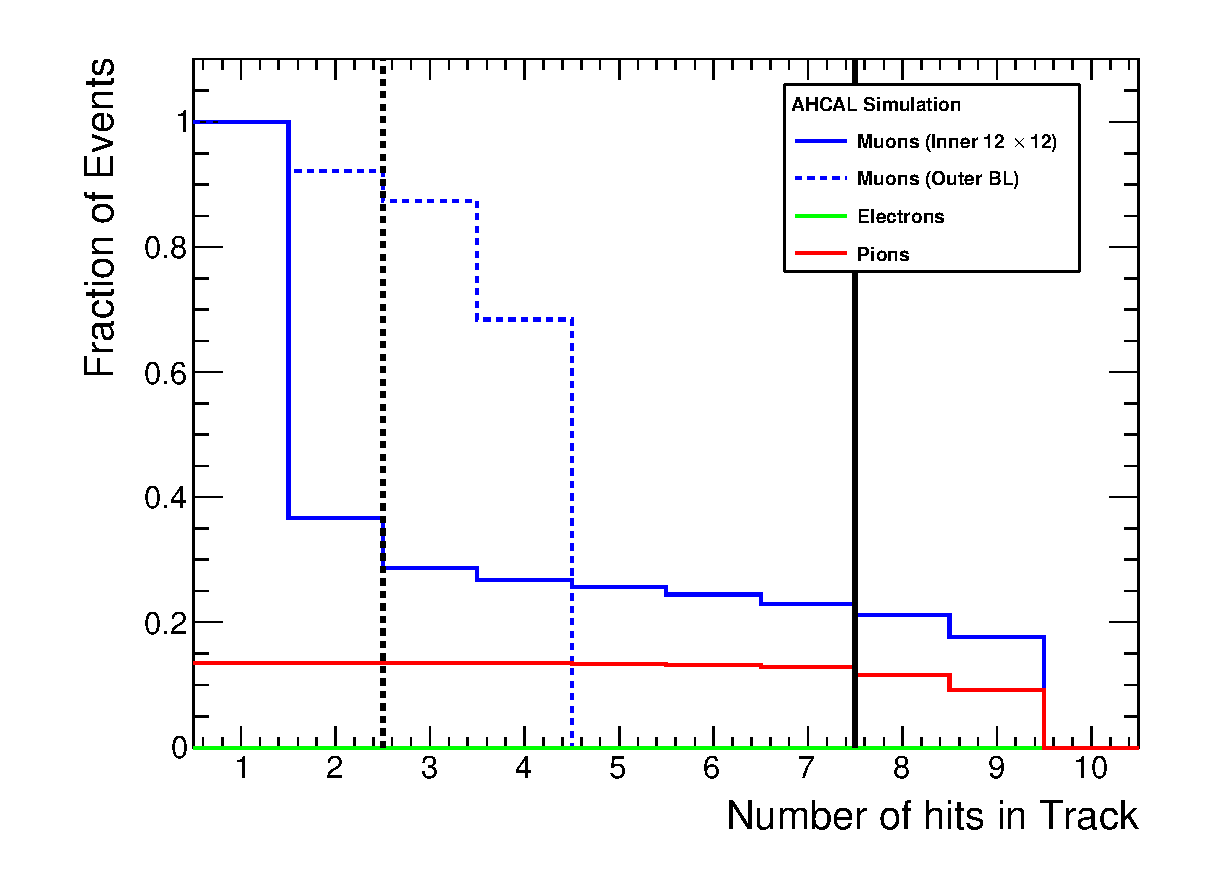
\includegraphics[width=1\linewidth]{../Thesis_Plots/Timing/Muons/Plots/TrackFinderCut_nHitsTrack_Muons.eps}
		\caption{} \label{fig:Muons_Track_nHits}
	\end{subfigure}
	\caption{\subref{fig:Muons_Track_nHitsLayer}) Distribution of number of hits in a layer normalized to the number of events for simulated muons at 150 GeV, electrons and pions at 50 GeV. The black line represents the cut of the maximum allowed number of hits in a layer applied for the MIP selection. \subref{fig:Muons_Track_nHits}) Distribution of the number of hits in a track normalized to the number of events for simulated muons at 150 GeV, electrons and pions at 50 GeV. A AHCAL tower size cut of 7 hits for the inner 12 $\times$ 12 tiles and a AHCAL tower size of 2 hits for the layers 11 to 14 on the outer tiles (Outer BL) were chosen.}
\end{figure}

\subsection{Electron Selection}
\label{subsec:elec_sel}

The electron selection is done to extract single electron showers contained in the AHCAL. These events are needed to validate the timing behavior in simulation as well as the detector simulation model as explained in chapter \ref{chap:TimingValidation}. It is important to have a clean sample of electrons to cross-check the timing calibration. For the selection, an \textit{Event Quality} pre-selection is done using the beam instrumentation and layer information. Events with a Cherenkov tag (only applied to data) are used. The distributions of the energy deposit in the first three AHCAL layers ($E_3+E_4+E_5$) are shown in figures \ref{fig:e10GeV_E3} and \ref{fig:e50GeV_E3} for simulated muon, electron and pion beams. In order to suppress muons and pions, $E_3+E_4+E_5$ must be over 10 MIPs.

In a next step, the electron selection is performed. Usually, one could use a shower start algorithm to select electrons that interact in the first layers of the calorimeter and reject pions efficiently \cite{Hartbrich:2016bbz}. However, the first ECAL layers (see section \ref{subsec:ScECAL}) can't be used because of high noise and the detector is partially equipped with active layers. This would greatly influence the performance of such algorithm, therefore, an alternative selection is needed.

A cut on the number of hits per event ($n_{Hits}$) versus the center of gravity in z ($CoG_Z$) is done. It is shown in figures \ref{fig:e10GeV_nHitsCoGZ} and \ref{fig:e50GeV_nHitsCoGZ}. The box cut in the figures does not induce any bias for the timing study in this thesis, it would only reduce the event statistics. In addition, the number of hits in a electron shower is proportional to the shower energy, thus this cut is energy dependent.

Finally, a cut on the energy deposited in the last two layers relative to the energy deposited in the calorimeter ($(E_{13}+E_{14})/\Sigma E$) is done. The distributions are shown in figures \ref{fig:e10GeV_Elast} and \ref{fig:e50GeV_Elast}. This cut is required to be under 1\% to reject pion showers and to contain the electron shower.

Additionally, to reduce transverse leakage, the shower center of gravity in X and Y needs to be within -90 mm and 90 mm. This cut is wider than the trigger scintillator but has no significant impact. The selection efficiencies for muon, electron and pion beams are shown in table \ref{table:eff_electron} for different beam energies from 10 GeV to 50 GeV. The detailed selection cuts are summarized in appendix table \ref{table:electron_sel}.

\begin{table}[htb!]
	\centering
	\caption{Efficiency of the electron selection for simulated electrons, muons and pions for energies between 10 and 50 GeV. The efficiency is defined as the number of events after selection over the number of event before selection.}
	\label{table:eff_electron}
	\begin{tabular}{@{} llll @{}}
		\toprule
		\textbf{Beam Energy} & \textbf{$\epsilon_{\mu}$} & \textbf{$\epsilon_{e}$} & \textbf{$\epsilon_{\pi}$}\\
		\midrule
		10 GeV & <0.1\% & 96\% & 15.9\%\\
		15 GeV & <0.1\% & 95.7\% & 10.1\%\\
		20 GeV & <0.1\% & 95.2\% & 6.3\%\\
		30 GeV & <0.1\% & 93.9\% & 2.3\%\\
		40 GeV & <0.1\% & 92.7\% & 1.2\%\\
		50 GeV & <0.1\% & 91.5\% & 1.1\%\\
		\bottomrule
	\end{tabular}
\end{table}

One can notice from table \ref{table:eff_electron} that a significant fraction of pions is present at low beam energies (10 to 20 GeV). But as the production of electrons in the beamline was done using a beam of photons on a beryllium target, it is with confidence that there is no pion contamination in the data \cite{AmbraEnergy}. Thus no additional cut is needed.

\begin{figure}[htbp!]
	\begin{subfigure}[t]{0.49\textwidth}
		\centering
		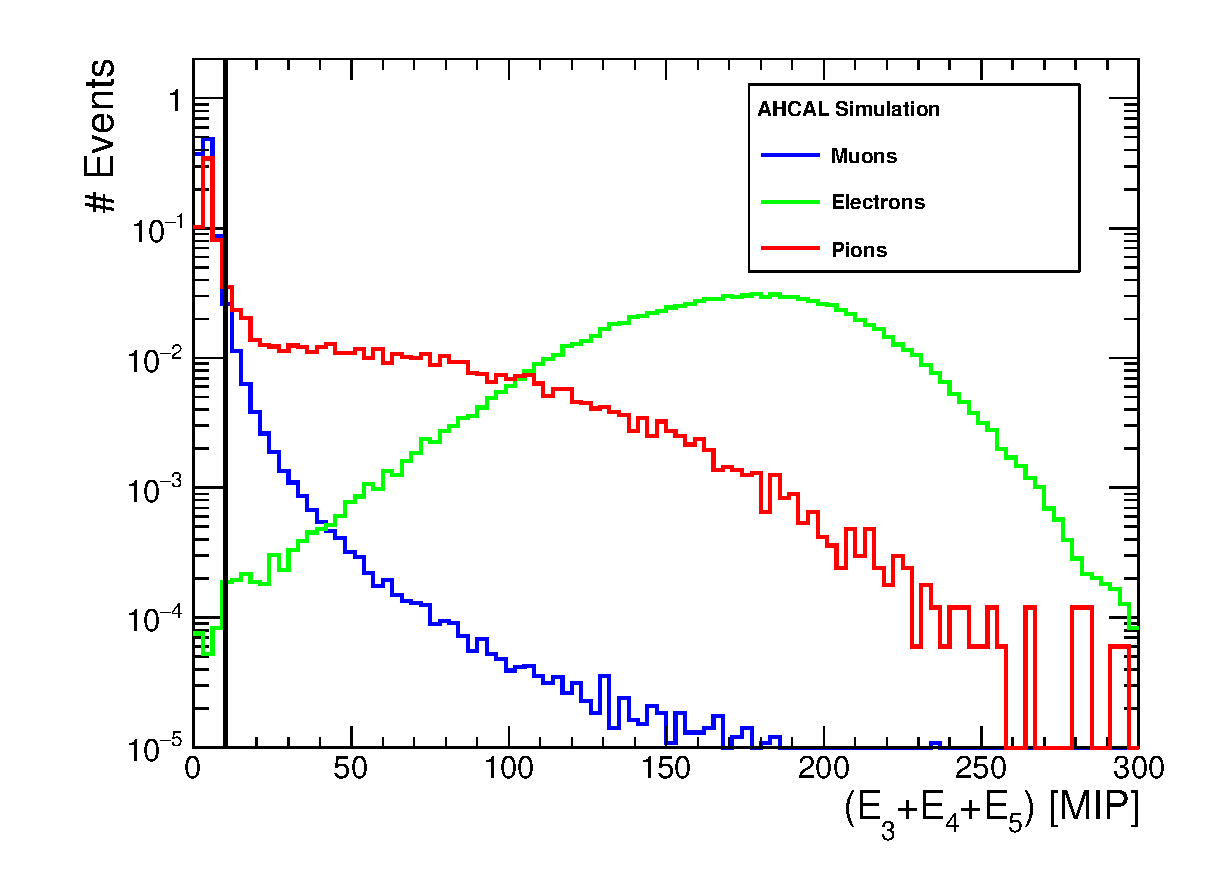
\includegraphics[width=1\linewidth]{../Thesis_Plots/Timing/Electrons/Plots/SelectionCut_EnergyE3_10GeV.eps}
		\caption{10 GeV.} \label{fig:e10GeV_E3}
	\end{subfigure}
	\hfill
	\begin{subfigure}[t]{0.49\textwidth}
		\centering
		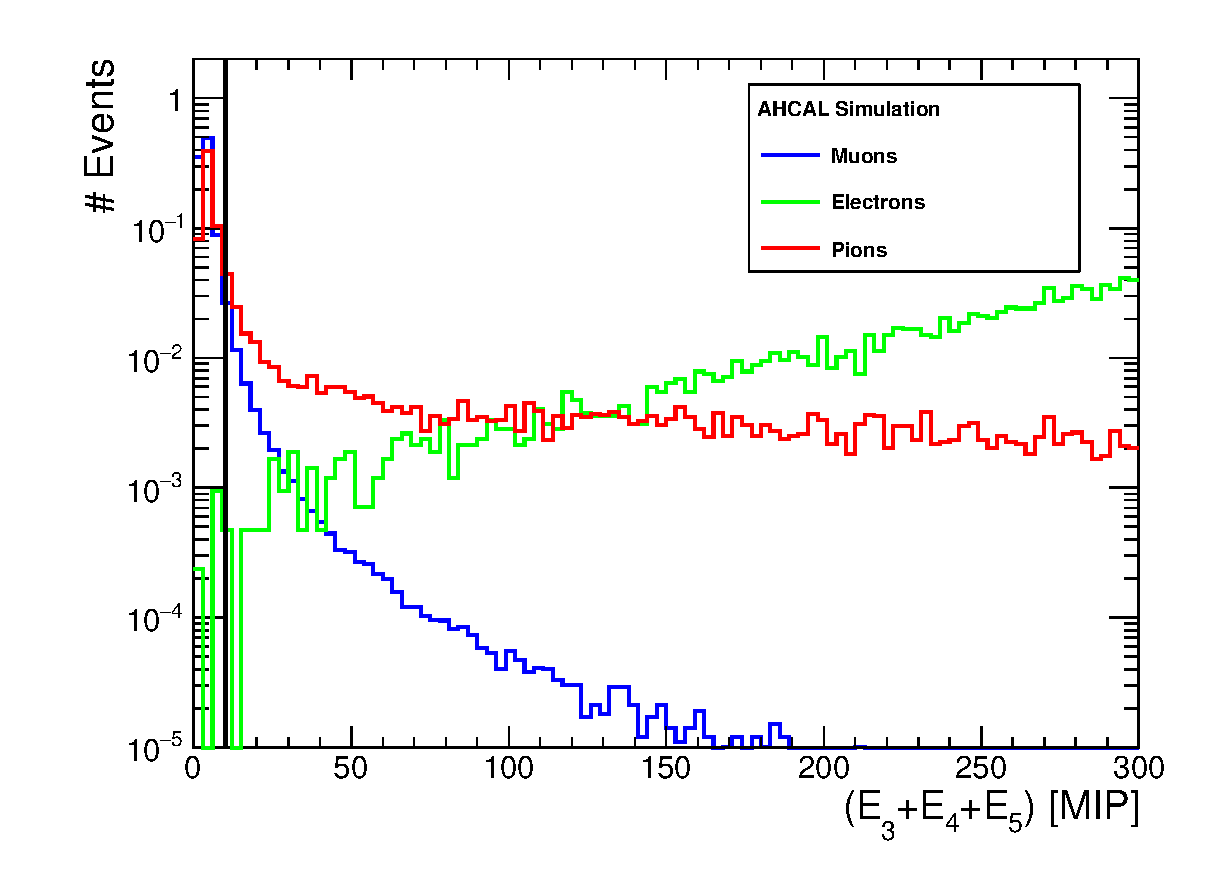
\includegraphics[width=1\linewidth]{../Thesis_Plots/Timing/Electrons/Plots/SelectionCut_EnergyE3_50GeV.eps}
		\caption{50 GeV.} \label{fig:e50GeV_E3}
	\end{subfigure}
	\hfill
	\begin{subfigure}[t]{0.5\textwidth}
		\centering
		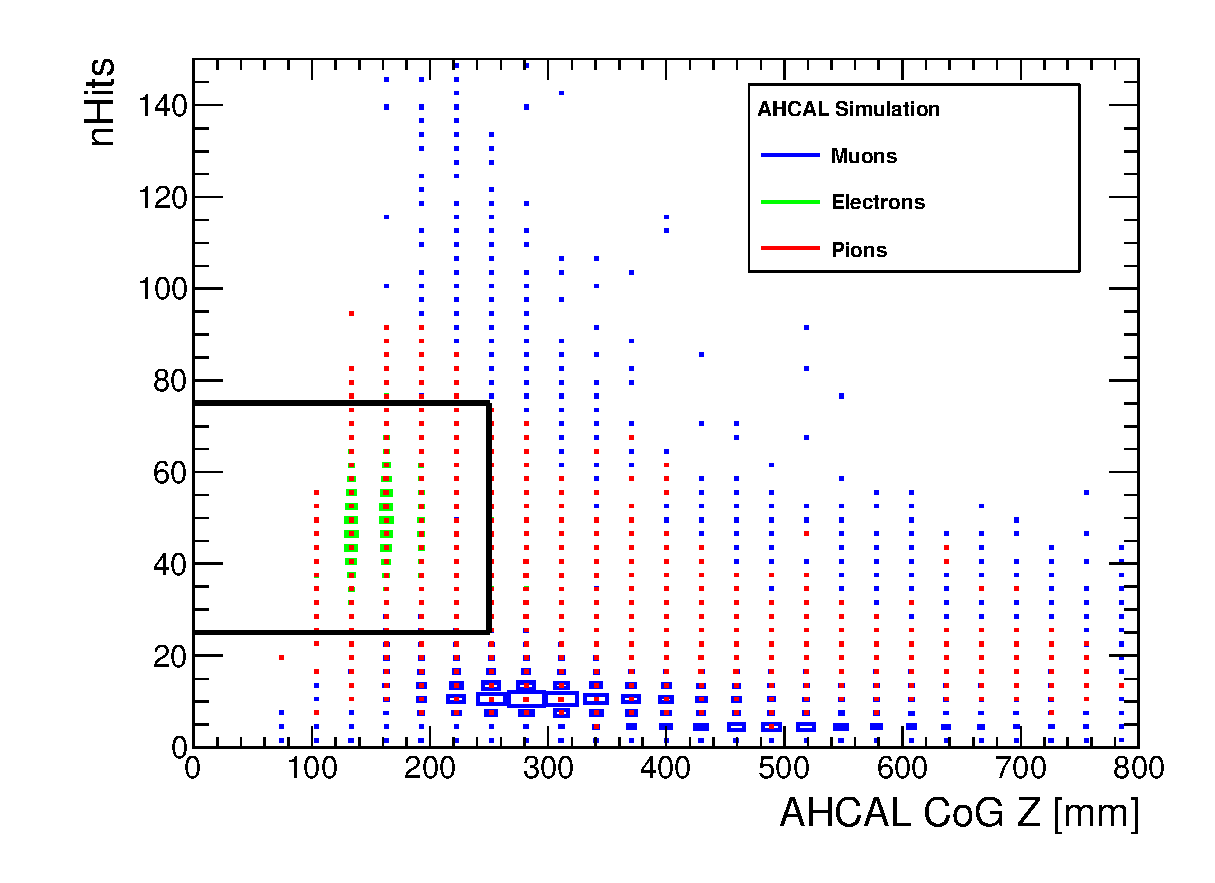
\includegraphics[width=1\linewidth]{../Thesis_Plots/Timing/Electrons/Plots/SelectionCut_nHitsCoGZ_10GeV.eps}
		\caption{10 GeV.} \label{fig:e10GeV_nHitsCoGZ}
	\end{subfigure}
	\hfill
	\begin{subfigure}[t]{0.5\textwidth}
		\centering
		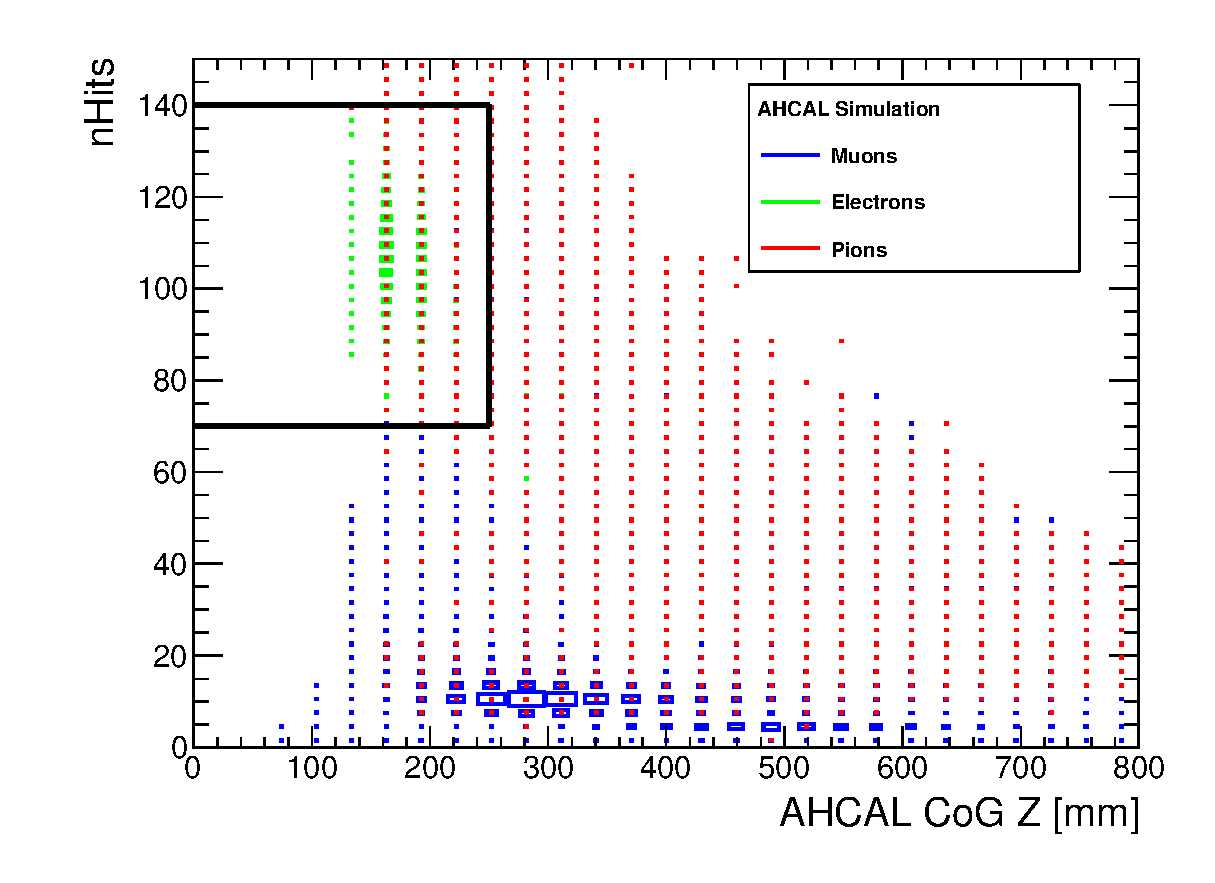
\includegraphics[width=1\linewidth]{../Thesis_Plots/Timing/Electrons/Plots/SelectionCut_nHitsCoGZ_50GeV.eps}
		\caption{50 GeV.} \label{fig:e50GeV_nHitsCoGZ}
	\end{subfigure}
	\hfill
	\begin{subfigure}[t]{0.5\textwidth}
		\centering
		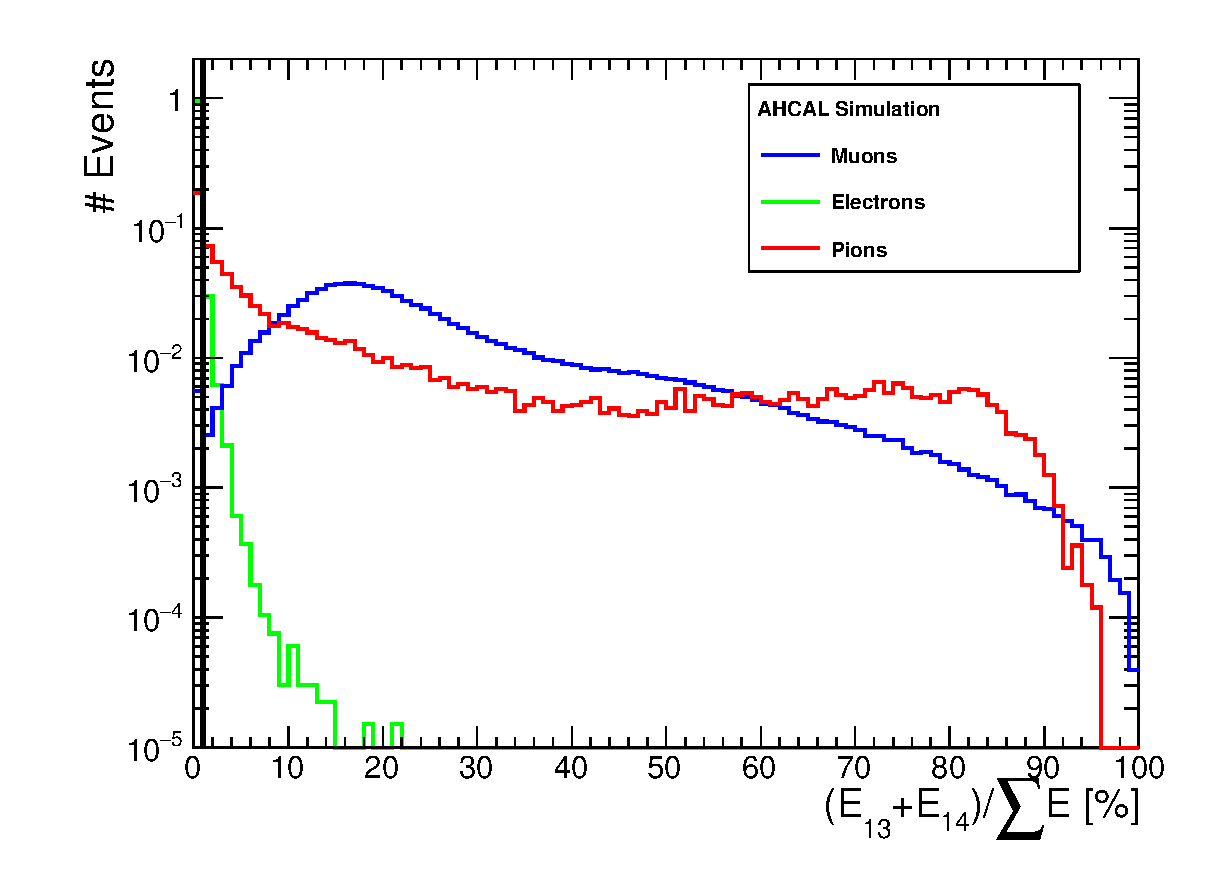
\includegraphics[width=1\linewidth]{../Thesis_Plots/Timing/Electrons/Plots/SelectionCut_EnergyLastLayers_10GeV.eps}
		\caption{10 GeV.} \label{fig:e10GeV_Elast}
	\end{subfigure}
	\hfill
	\begin{subfigure}[t]{0.5\textwidth}
		\centering
		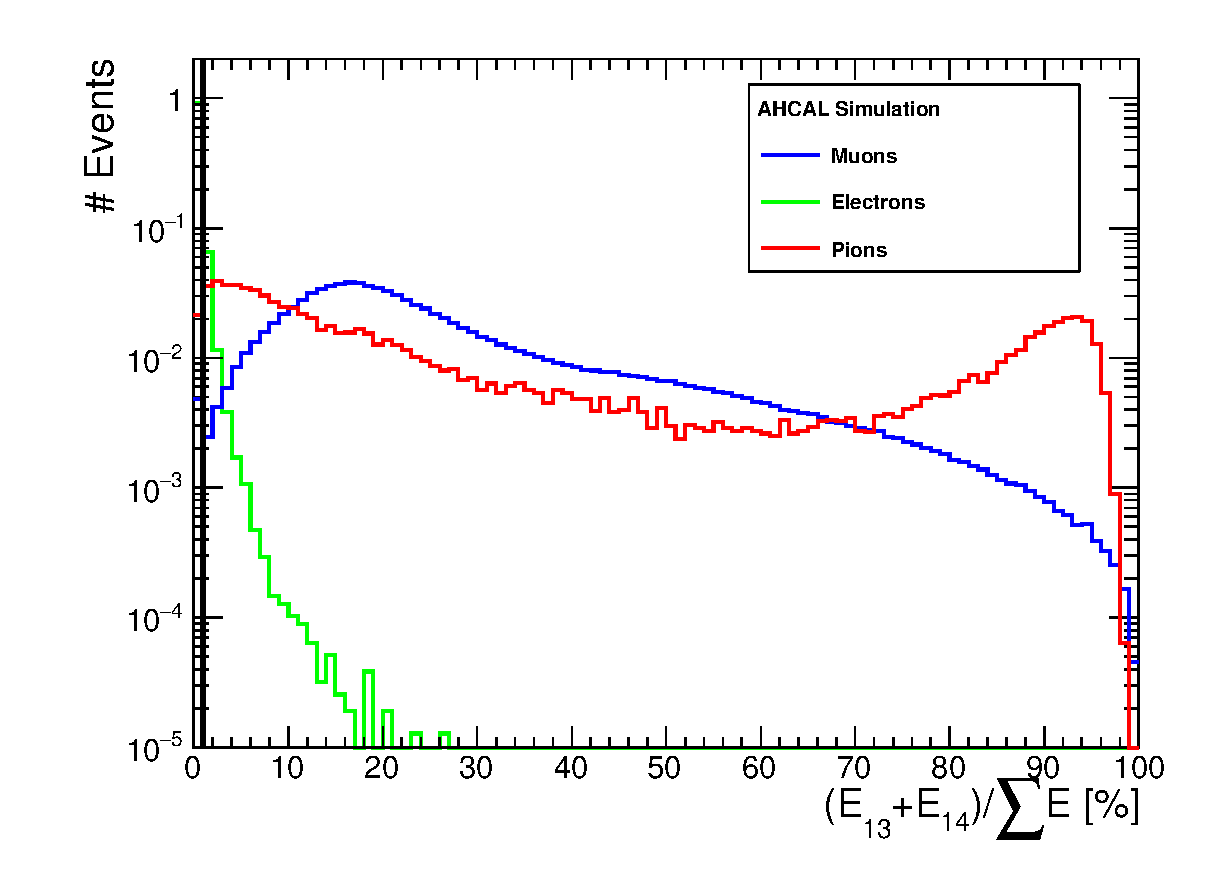
\includegraphics[width=1\linewidth]{../Thesis_Plots/Timing/Electrons/Plots/SelectionCut_EnergyLastLayers_50GeV.eps}
		\caption{50 GeV.} \label{fig:e50GeV_Elast}
	\end{subfigure}
	\caption{Distribution of the variables used in the electron selection of simulated electron and pion beams between 10 and 50 GeV. The muons are simulated at 150 GeV. These plots were used to determine the best selection criteria for electrons.} \label{fig:electronselection}
\end{figure}

\subsection{Pion Selection}
\label{sec:pionsel}

The goal of the pion selection is to reject punch-through pions, muons and possible electron contamination as these events would be instantaneous (see section \ref{sec:TimeDevShowers}). An \textit{Event Quality} pre-selection is performed using the Cherenkov information. The events without a Cherenkov tag are selected. This is only applied to data. The pion selection is based on the same variables as the electron selection: $cog_Z:n_{Hits}$ plane, $(E_{13}+E_{14})/\Sigma E$ and additionally the number of hits in two first AHCAL layers ($N_3+N_4$).

Firstly, the distribution of events in the $cog_Z:n_{Hits}$ plane is shown in figures \ref{fig:pi10GeV_nHitsCoGZ} and \ref{fig:pi90GeV_nHitsCoGZ} for muon, electron and pion beam energies from 10 GeV to 90 GeV. The number of hits required per event needs to be over 20 to reject most muons or punch-through pions without cutting on the center of gravity in z in order not to bias the start of the pion shower.

Secondly, the distributions of the energy fraction deposited in the two last AHCAL layers are shown in figures \ref{fig:pi10GeV_Elast} and \ref{fig:pi90GeV_Elast}. This variable must be over 1\% in order to ensure that pion showered and reject electrons. Finally, the distributions of the number of hits in the two first AHCAL layers is shown in figure \ref{fig:pi10GeV_N3N4} and \ref{fig:pi90GeV_N3N4}. The number of hits in the two first AHCAL layers must be under 5 to mitigate possible particle contamination from electrons.

The selection efficiencies for muon, electron and pions beams for different beam energies between 10 and 90 GeV are shown in table \ref{table:eff_pion}. At 10 GeV, one can observe a low pion selection efficiency that is due to the fact less energy is deposited in the last two layers of the AHCAL thus reducing the number of selected pion events.

\begin{table}[htb!]
	\centering
	\caption{Efficiency of the pion selection for beam energies between 10 and 90 GeV. The efficiency is defined as the number of events after selection over the number of event before selection.}
	\label{table:eff_pion}
	\begin{tabular}{@{} llll @{}}
		\toprule
		\textbf{Beam Energy} & \textbf{$\epsilon_{\mu}$} & \textbf{$\epsilon_{e}$} & \textbf{$\epsilon_{\pi}$}\\
		\midrule
		10 GeV & <0.1\% & <0.1\% & 29.9\%\\
		30 GeV & 0.9\% & <0.1\% & 50.3\%\\
		50 GeV & 0.9\% & <0.1\% & 51.1\%\\
		70 GeV & 0.9\% & <0.1\% & 51\%\\
		90 GeV & 0.9\% & <0.1\% & 50.2\%\\
		\bottomrule
	\end{tabular}
\end{table}

In addition, multiple particle events were observed in the data as shown in figure \ref{fig:DoubleParticleEvent}. As no beam instrumentation could be used for rejecting these events, a rejection method based on the hit time information was developed.

\begin{figure}[htbp!]
	\centering
	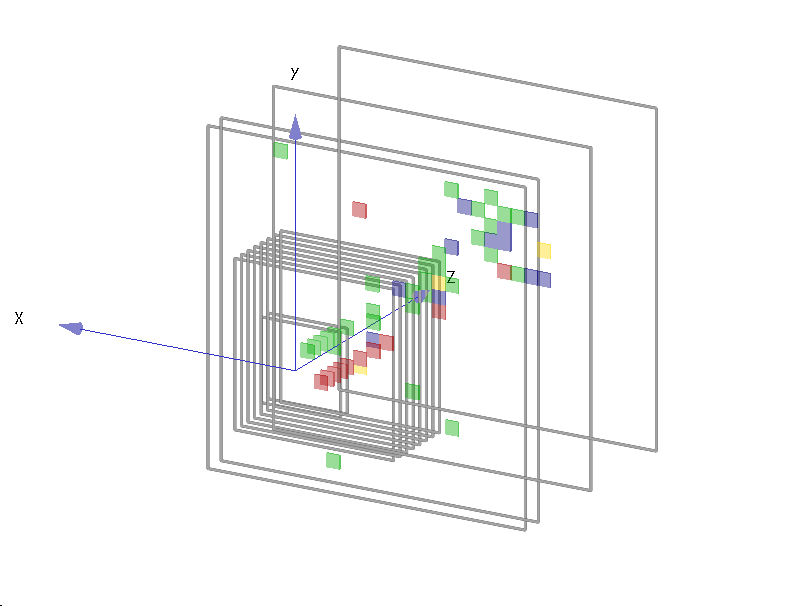
\includegraphics[width=0.7\linewidth]{chap5/fig_AHCAL_timing/Pions/DoubleParticleEventPions.png}
	\caption{Multi-particle event in the 50 GeV pion data sample. The colors represent the time of the hit: green < 5 ns, blue 5 ns to 15 ns, yellow 15 ns to 35, orange 35 ns to 50 ns and red > 50 ns. One can observe an additional late muon going through the detector.} \label{fig:DoubleParticleEvent}
\end{figure}

The method is the following: all the hits in an event are placed and ordered in time; Then for each hit after 50 ns, a timing window of 30 ns used. The number of hits in that window are counted. If the number of hits is larger than 5, it is classified as a \textit{late cluster}. The event is rejected if there is at least one late cluster. This method works because if an event has several particles, the time reference of the event is generated by the first particle. Therefore, the second particle will have all the hits late relative to the time reference and thus the event will be rejected.

The method is based on data in order to remove multi-particle events. The multi-particle event rejection has been checked on simulated data and affects the selection between <0.1\% up to 2\% from 10 to 90 GeV pions. These multi-particle events are greatly suppressed in data. The number of events removed varies between 0.1\% and 1\% depending on the beam energy. Due to the calorimeter not being fully equipped thus providing limited information, some contamination may remain in the data.

A detailed description of the selection cuts are shown in appendix table \ref{table:pion_sel}.

\begin{figure}[htbp!]
	\begin{subfigure}[t]{0.49\textwidth}
		\centering
		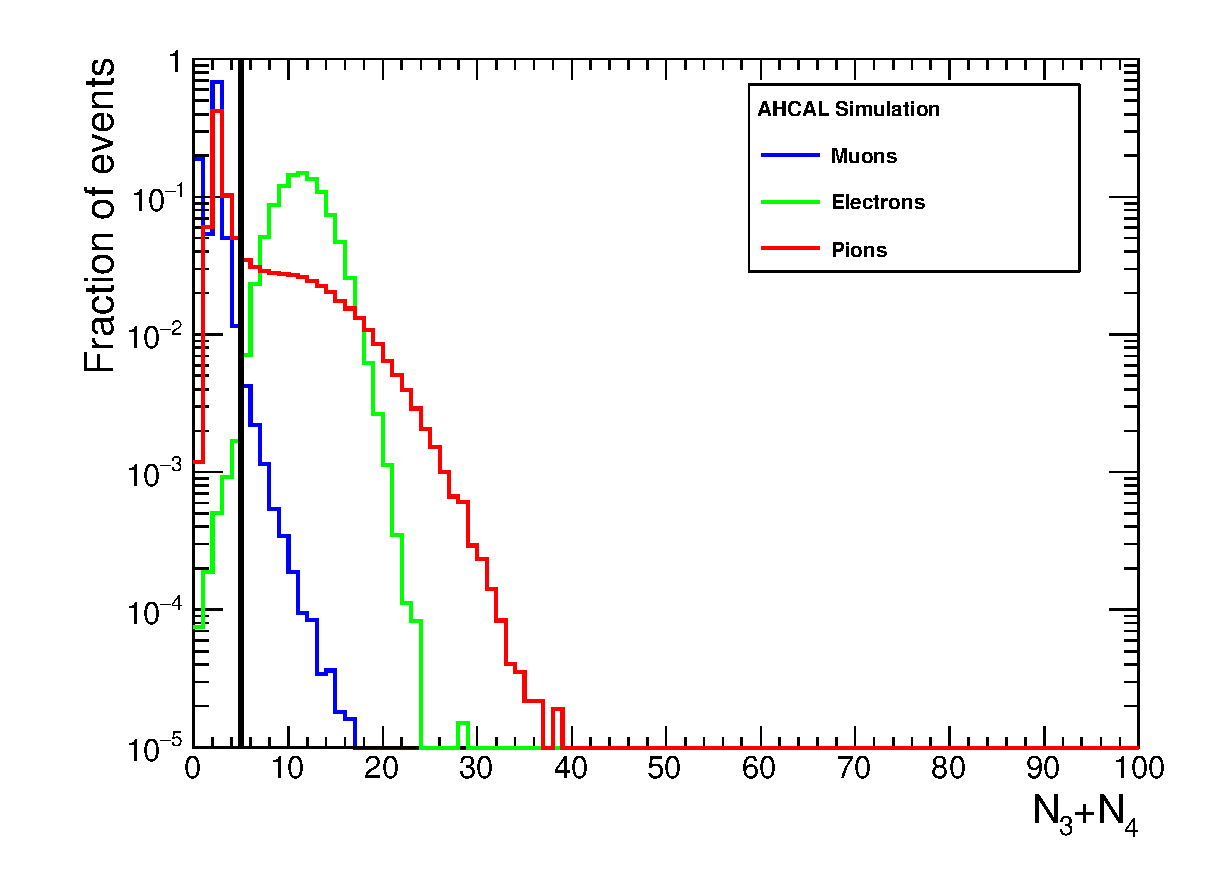
\includegraphics[width=1\linewidth]{../Thesis_Plots/Timing/Pions/Plots/SelectionCut_N3N4_10GeV.eps}
		\caption{10 GeV.} \label{fig:pi10GeV_N3N4}
	\end{subfigure}
	\hfill
	\begin{subfigure}[t]{0.49\textwidth}
		\centering
		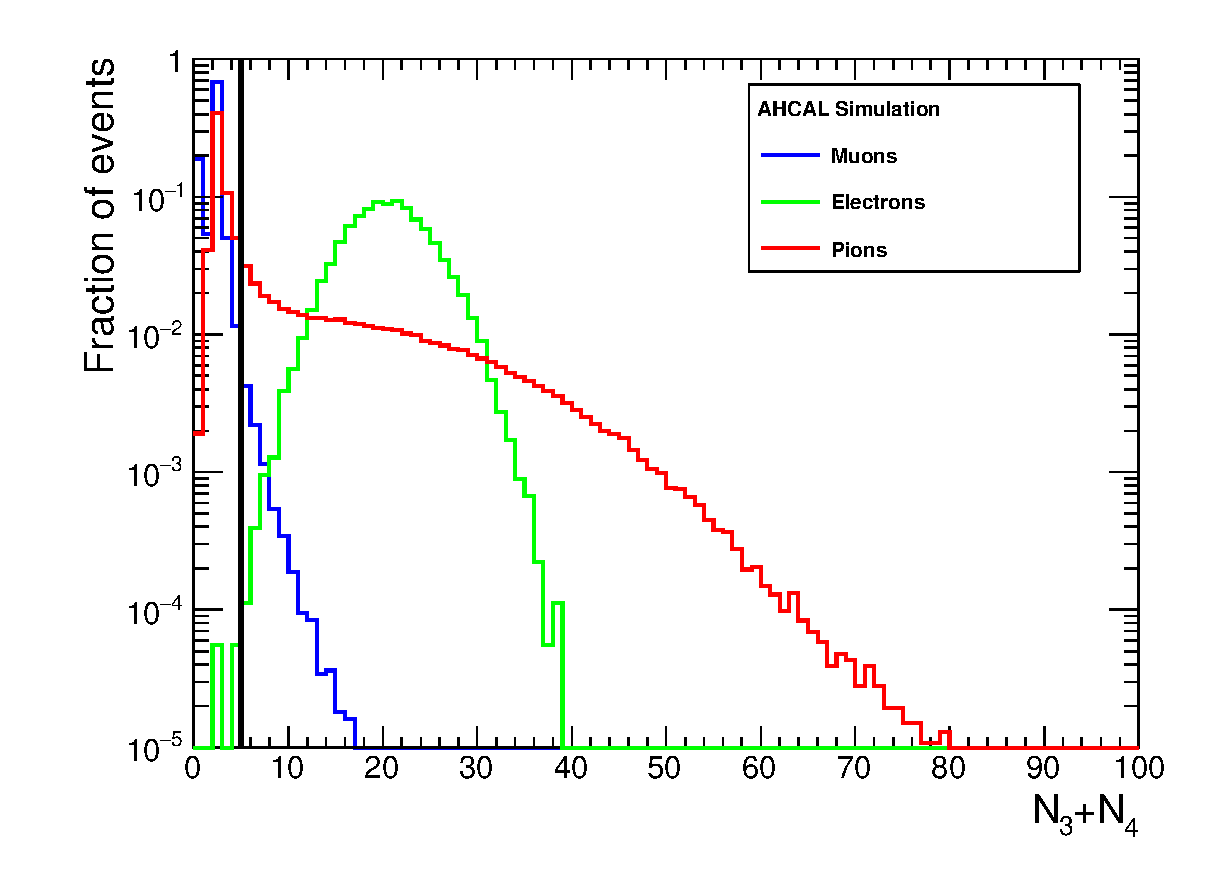
\includegraphics[width=1\linewidth]{../Thesis_Plots/Timing/Pions/Plots/SelectionCut_N3N4_90GeV.eps}
		\caption{90 GeV.} \label{fig:pi90GeV_N3N4}
	\end{subfigure}
	\hfill
	\begin{subfigure}[t]{0.49\textwidth}
		\centering
		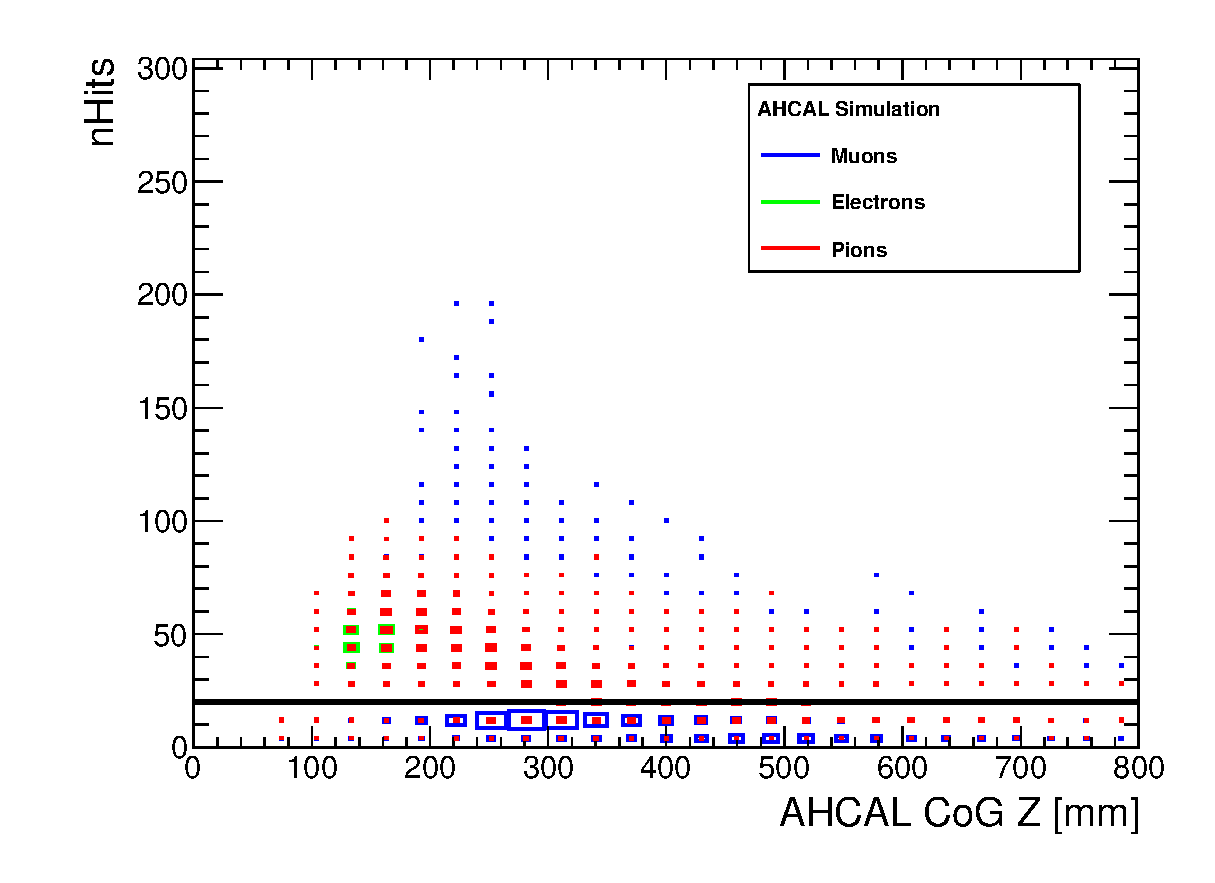
\includegraphics[width=1\linewidth]{../Thesis_Plots/Timing/Pions/Plots/SelectionCut_nHitsCoGZ_10GeV.eps}
		\caption{10 GeV.} \label{fig:pi10GeV_nHitsCoGZ}
	\end{subfigure}
	\hfill
	\begin{subfigure}[t]{0.49\textwidth}
		\centering
		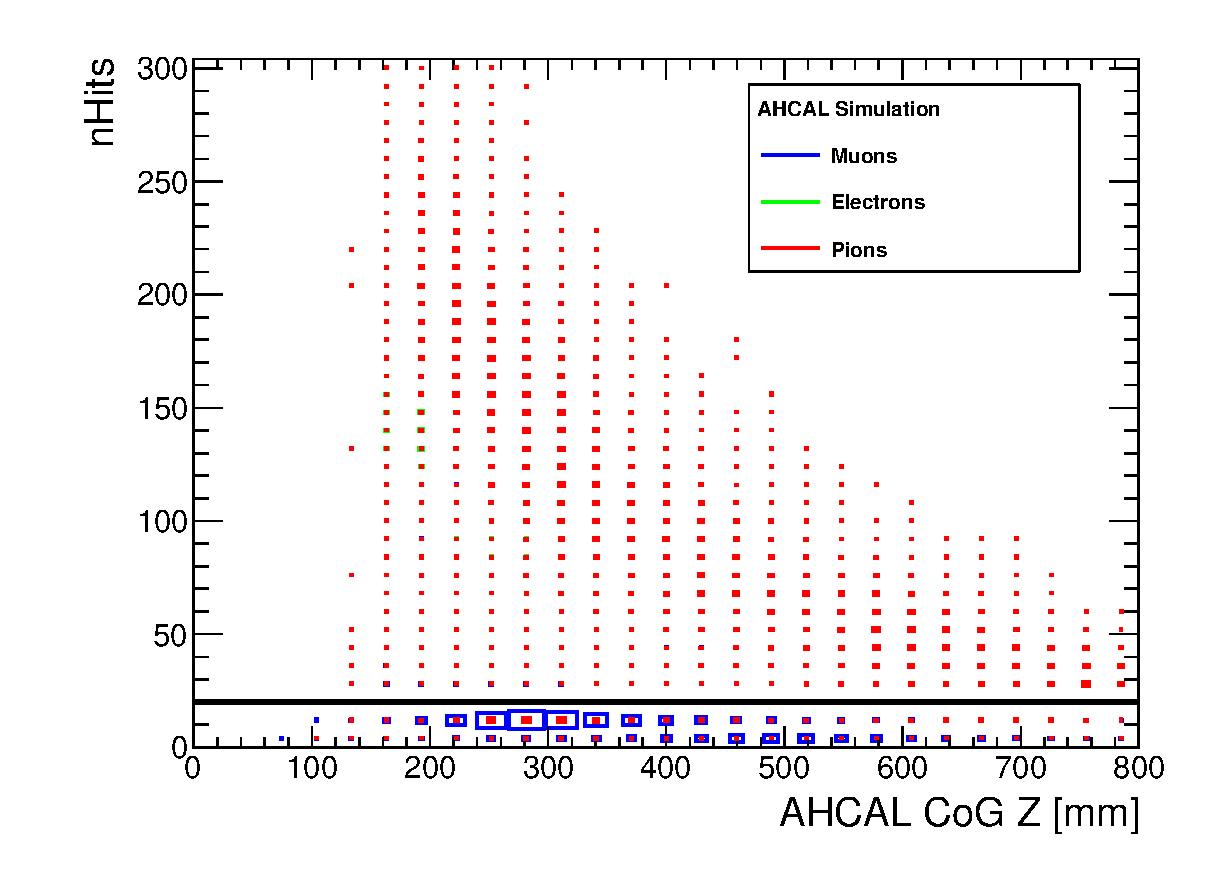
\includegraphics[width=1\linewidth]{../Thesis_Plots/Timing/Pions/Plots/SelectionCut_nHitsCoGZ_90GeV.eps}
		\caption{90 GeV.} \label{fig:pi90GeV_nHitsCoGZ}
	\end{subfigure}
	\hfill
	\begin{subfigure}[t]{0.49\textwidth}
		\centering
		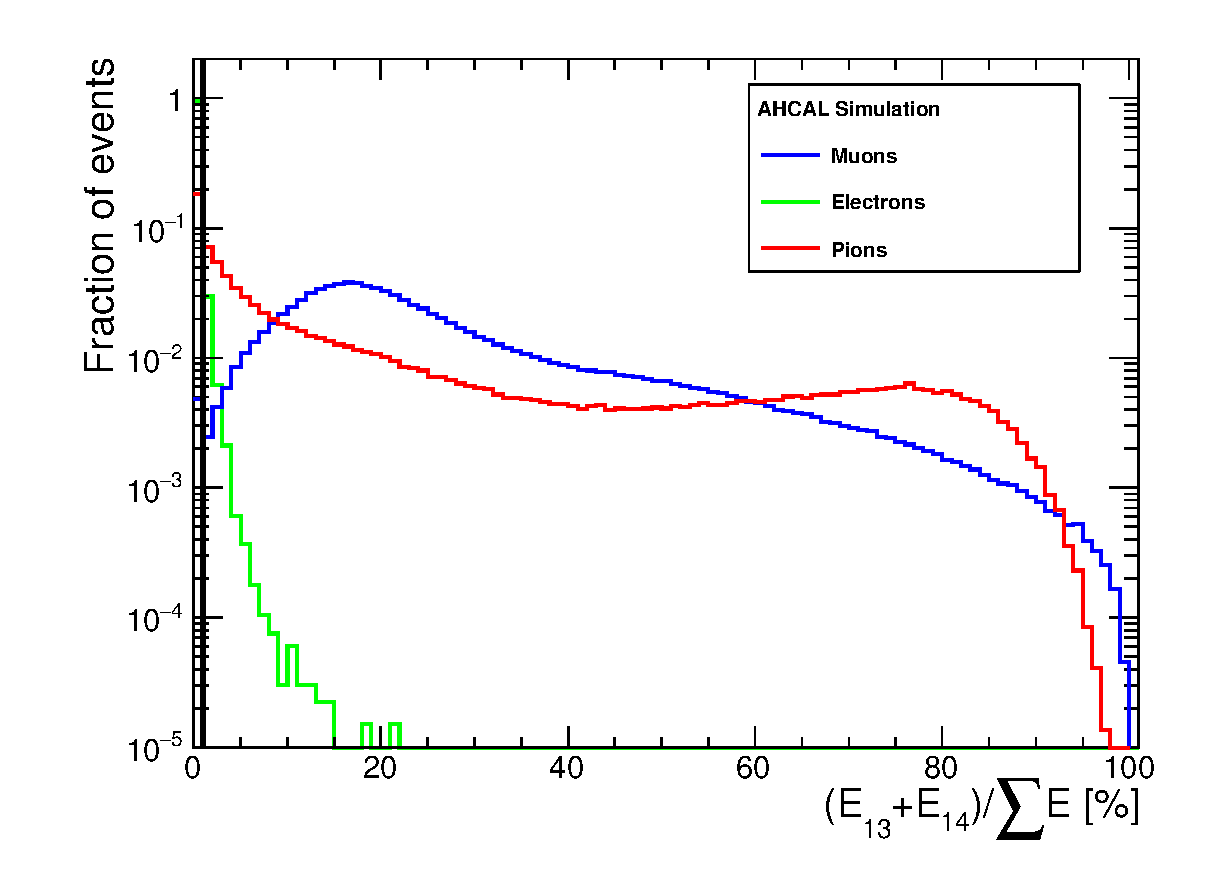
\includegraphics[width=1\linewidth]{../Thesis_Plots/Timing/Pions/Plots/SelectionCut_EnergyLastLayers_10GeV.eps}
		\caption{10 GeV.} \label{fig:pi10GeV_Elast}
	\end{subfigure}
	\hfill
	\begin{subfigure}[t]{0.49\textwidth}
		\centering
		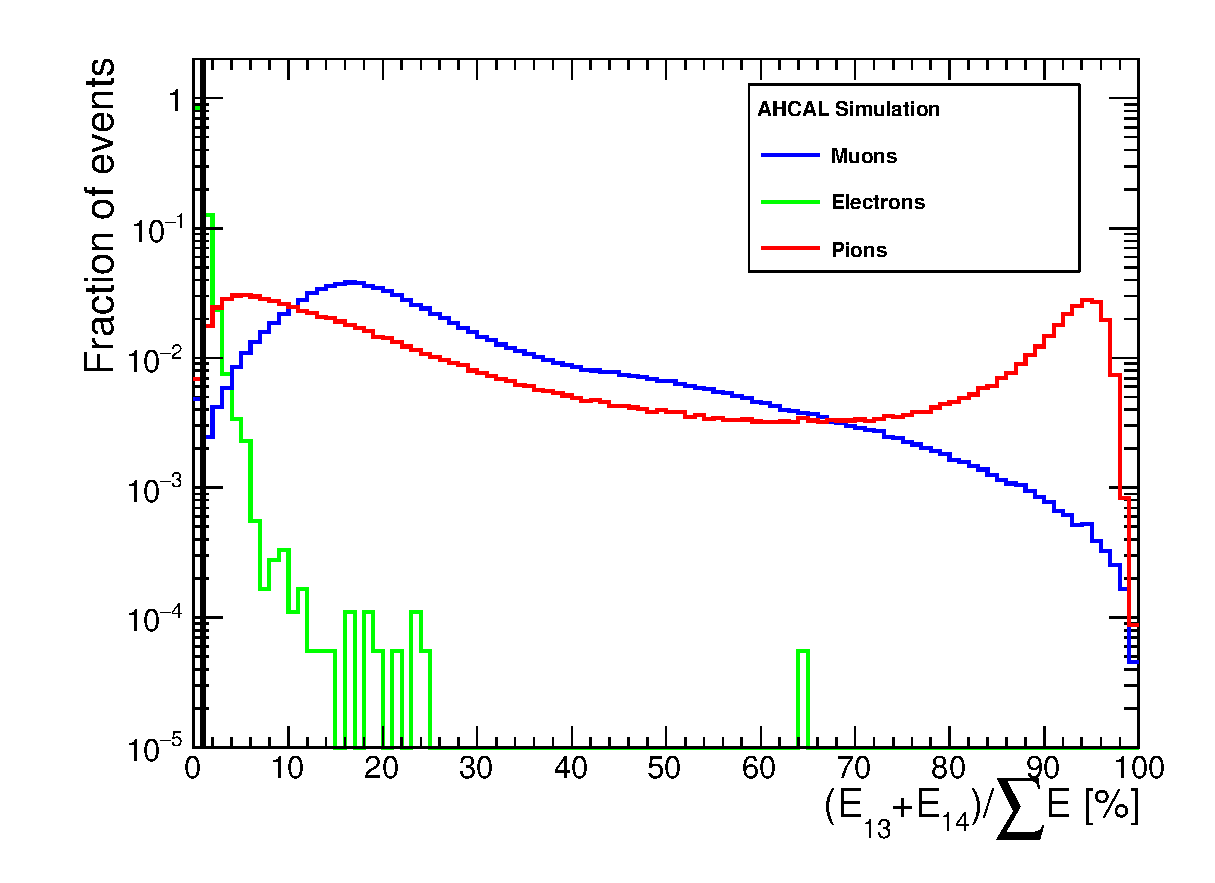
\includegraphics[width=1\linewidth]{../Thesis_Plots/Timing/Pions/Plots/SelectionCut_EnergyLastLayers_90GeV.eps}
		\caption{90 GeV.} \label{fig:pi90GeV_Elast}
	\end{subfigure}
	\caption{Distribution of the variables used in the pion selection for simulated muon, electron and pion beams between 10 and 90 GeV. Theses plots were used to determine the best selection criteria for pions.} \label{fig:pionselection}
\end{figure}

\subsection{Rejection of outlier chips}
\label{sec:ChipRejection}

A careful check of the time of first hit distribution (see chapter \ref{chap:TimingCalib}) for each chip has been performed to reject any outlier. For all the data collected, the layer 11 is rejected due to a likely problem with the electronics (see section \ref{subsec:slope_calib}). For the muon data, a single chip (157) shows a strange behavior likely because the input DAC on this chip is broken resulting in an unstable voltage applied to the SiPM.

\begin{figure}[htbp!]
	\begin{subfigure}[t]{0.49\textwidth}
		\centering
		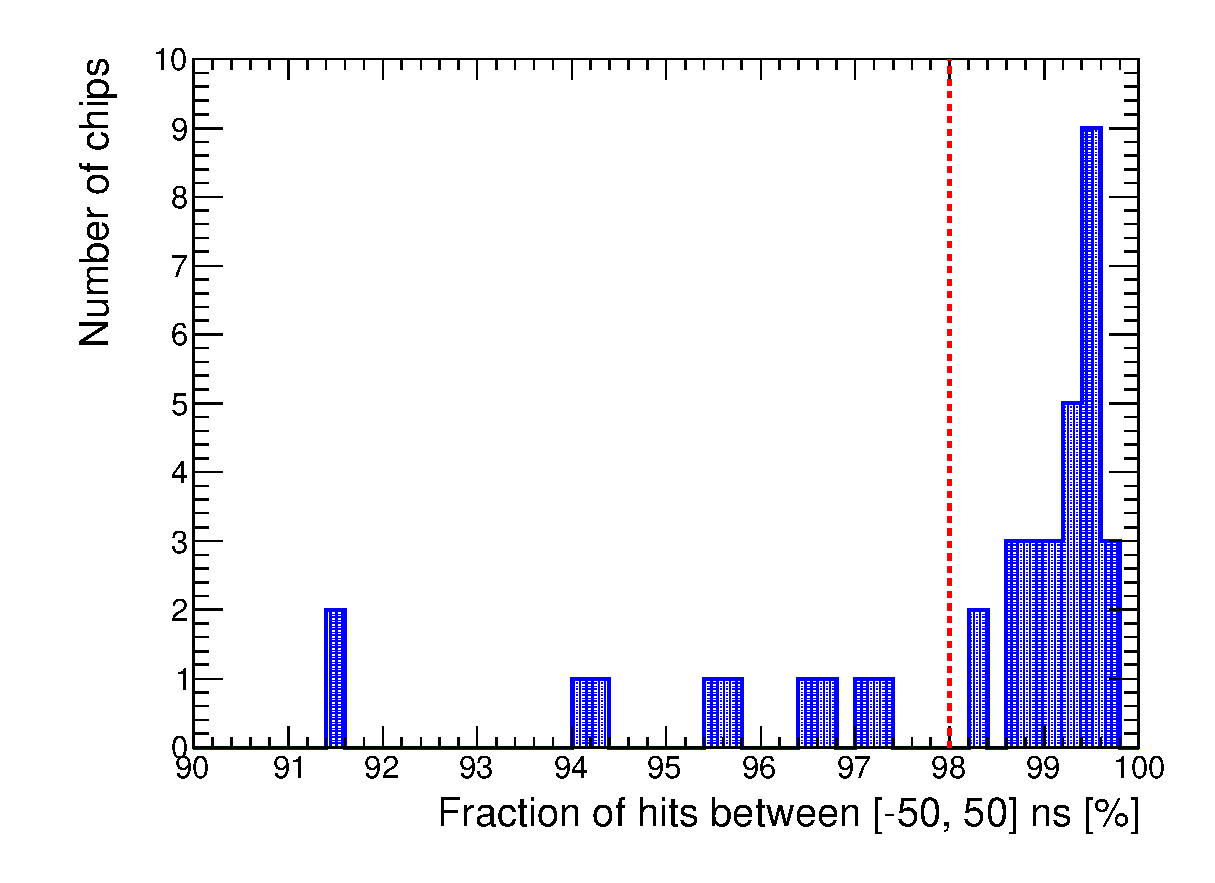
\includegraphics[width=1\linewidth]{../Thesis_Plots/Timing/Electrons/Plots/FractionRejectedChips.eps}
		\caption{} \label{fig:FracRejChip}
	\end{subfigure}
	\hfill
	\begin{subfigure}[t]{0.49\textwidth}
		\centering
		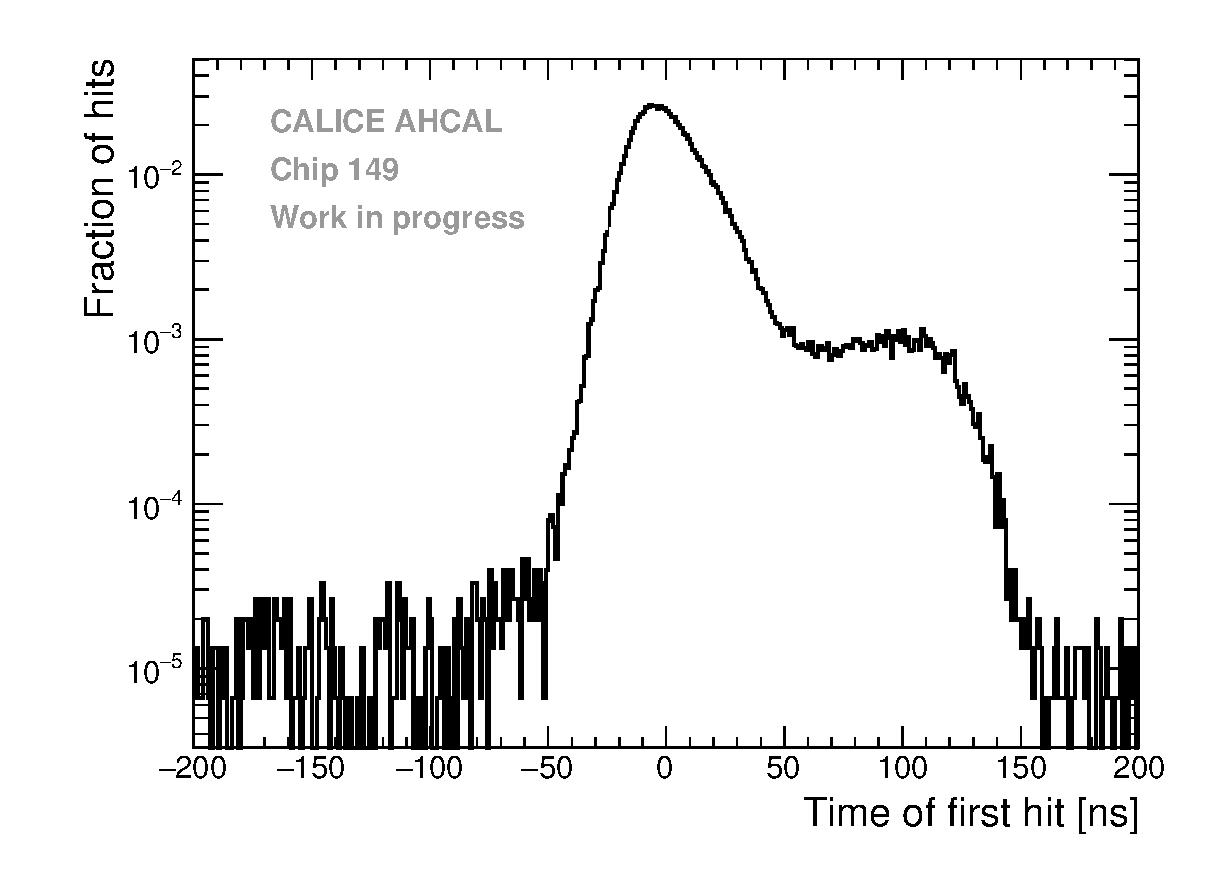
\includegraphics[width=1\linewidth]{../Thesis_Plots/Timing/Electrons/Plots/ExampleBadChip149.eps}
		\caption{} \label{fig:ExBadChip}
	\end{subfigure}
	\caption{\subref{fig:FracRejChip}) Distribution of the variable $R_{chip}$ for 50 GeV electrons for all chips. Each entry corresponds to a chip. The red line represent the cut applied to reject bad chips. \subref{fig:ExBadChip}) Example of a typical bad chip that is rejected with this method (Chip 149).}
\end{figure}

For the electron data, the variable $R_{chip}$ was used to determine bad behaving chips and it is calculated as
\begin{equation} \label{eq:fraction_rejection}
	R_{chip} = \frac{1}{N_{total}} \left| N_{50 ns}^{200 ns} - N_{-200 ns}^{50 ns} \right|
\end{equation}
where $N_{total}$ is the total number of entries, $N_{50 ns}^{200 ns}$ is the number of entries between 50 ns and 200 ns and $N_{-200 ns}^{50 ns}$ is the number of entries between -200 ns and 50 ns. The variable is minimum when most of the hits in the chip are outside of the core of the time distribution between -50 and 50 ns. If $R$ is below 98\%, the chip is rejected. With this method, 20 chips are rejected.

For the pion data, applying the same method as for electrons is not possible due to a late tail to higher time related to delayed energy depositions from neutrons. The same chips as for electrons were rejected but in addition, each chip time distribution after correction were manually checked. The chips that presented an abnormal shape such as double peaks were discarded. Hence, 16 chips are additionally rejected. This leaves 44 chips in the pion analysis. A detailed table of the rejected chips can be seen in appendix \ref{appendix:rejection}.

\newpage
\begin{center}
  \rule{0.5\textwidth}{.4pt}
\end{center}

The datasets used for this thesis, the selection criteria for each beam type have been presented. MIP-like particles can be selected efficiently at more than 70\%. The electron selection has an efficiency of more than 90\% at all electron beam energies. The pion selection selects pions with an efficiency over 50\% for all pion energies except for 10 GeV where the selection efficiency is around 30\%. Multi-particle events in the pion data is observed. A method using the hit time information is used to mitigate these events. Up to 1\% of events can be removed. To be able to do a meaningful comparison of the data to simulations, accurate data calibration factors and a realistic AHCAL simulation model are essential. In the next chapter, the energy scale calibration of the AHCAL prototype and the validation of the AHCAL simulation model is presented.
